% MDPI Robotics submission, on the official MDPI class (2026-09-11). Build:
%   export PATH="/Library/TeX/texbin:$PATH"
%   pdflatex main && bibtex main && pdflatex main && pdflatex main
%
% Every number traces to a committed result JSON named in its table caption;
% scripts/print_paper_tables.py regenerates the amortization table rows from
% results_morph_3seed.json.

\documentclass[robotics,article,submit,moreauthors]{Definitions/mdpi}

\firstpage{1}
\makeatletter\setcounter{page}{\@firstpage}\makeatother
\pubvolume{1}
\issuenum{1}
\articlenumber{0}
\pubyear{2026}
\copyrightyear{2026}
\datereceived{ }
\dateaccepted{ }
\datepublished{ }

\newcommand{\eg}{e.g.}

\Title{One Model, Many Arms: Amortized Multimodal Inverse Kinematics Across a Continuous Family of Soft Continuum Manipulators}

\Author{Adhvay Jagadeesh *}
\AuthorNames{Adhvay Jagadeesh}

\address{Independent Researcher (no institutional affiliation)}
\corres{Correspondence: adhvayjagadeesh@gmail.com}

\abstract{A learned inverse-kinematics (IK) model for a soft continuum arm is
trained for one arm. Yet no two fabricated soft arms are the same arm:
segment lengths, stiffness, and actuation gain vary by fabrication tolerance,
and a model fitted to one instance is silently wrong on the next. We ask
whether a single conditional diffusion model can amortize inverse
kinematics across a continuous family of soft arms---solving IK for
morphologies it never saw---and what makes that possible. On a
piecewise-constant-curvature pneumatic arm whose four segment lengths and
four curvature gains are each drawn per sample from a continuous box, a
diffusion model conditioned on the morphology vector reaches
$0.41\pm0.04\,$mm best-of-32 tip error with $100\%$ success on held-out
in-distribution morphologies (three seeds)---within $0.06\,$mm of
specialists trained on $5\times10^5$ samples of their own arm, with zero
samples of any specific arm. A controlled ablation
isolates the cause: the identical randomized data with the morphology
\emph{withheld} yields $12.7\pm0.2\,$mm and $12\%$ success, a $31\times$ gap.
A direct test shows what the withheld-morphology model learned instead:
every one of its samples is a correct solution for \emph{some} arm in the
family ($100\%$), almost never for the queried one ($0$--$2\%$)---it
learned the marginal over arms, which also explains why gain randomization
recovers nothing under dynamics-model change. Generalization is flat
across the training box and degrades gracefully just beyond it---to
$10$--$15\%$ past the edge when extrapolation enlarges the workspace,
$25$--$33\%$ when it shrinks it---before a sharp cliff. Deterministic and mixture-density regressors trained
on the same data do not amortize ($14$--$16\,$mm in-distribution),
because the morphology-conditioned inverse map is more multimodal, not
less. The amortized model recovers $0.96\pm0.01$ of each unseen arm's
enumerated solution modes, matching a specialist's recall at equal mode
count. We report the single-arm advantage, its redundancy mechanism, and the
limits of transfer under dynamics-model change, with three-seed
statistics on every headline comparison. Code, data, and per-experiment
result files are released.}

\keyword{soft robotics; continuum manipulators; inverse kinematics;
diffusion models; amortized inference; domain randomization; multimodal
learning}

\begin{document}

% =========================================================================
\section{Introduction}
% =========================================================================

A multi-segment pneumatic continuum arm with three chambers per segment has
more actuation degrees of freedom than task degrees of freedom: for a
four-segment arm, a 12-D actuation vector determines a 3-D tip position. The
inverse map is one-to-many, and its preimages are not a connected null
space---distinct arm shapes reach the same tip. A deterministic learned IK
regressor trained by motor babbling~\cite{giorelli2015neural} fits the
conditional \emph{mean} of this multimodal distribution and can return an
actuation that realizes none of the true solutions. A conditional diffusion
model~\cite{ho2020denoising,song2021denoising} learns the full conditional
distribution $p(\mathbf{q}\,|\,\text{target})$ and can sample every solution
mode. We establish below, with three-seed statistics, that this advantage is
real, that it is specifically a redundancy effect, and that it does not
survive a change of dynamics model.

Every learned soft-arm IK method we are aware of, including the single-arm
models we begin with, trains one model for one arm. This paper starts from the observation that
\emph{one arm} is a fiction. A soft manipulator is a fabricated object:
its segment lengths depend on assembly, its bending stiffness on material
batch and geometry (for a rod-backed arm stiffness goes as the fourth power
of diameter, so a $\pm4\%$ tolerance is a $\pm17\%$ stiffness range), and
its actuation gain on chamber or tendon geometry. Two arms built from the
same drawing are two different arms. A model that must be retrained for each
one---at $5\times10^5$ simulated samples per arm---is a model that does not
scale past the bench it was trained on.

The question is therefore whether a single model can \emph{amortize}
inverse kinematics across a family of arms: trained once on a continuous
distribution of morphologies, and asked to solve IK for a specific
morphology it never saw, given only that morphology's parameters as a
conditioning input. This is the soft-robotic instance of a question now
central to rigid-robot learning, where diffusion IK has been made to
generalize across kinematic-tree \emph{topologies}~\cite{zhang2025ikdiffuser,
limoyo2025generative}. Soft arms pose it differently: the morphology is not
a discrete topology but a continuous vector, and the conditional
distribution the model must represent is more multimodal, not less---the
same tip is reached by different shapes on different arms.

There is a specific reason to doubt the answer is yes. Domain randomization
(DR)~\cite{tobin2017domain}---training on randomized arm parameters so that
the model is robust to their variation---recovers \emph{nothing} under
model change in our experiments, while degrading in-domain accuracy
fivefold (Sec.~\ref{sec:transfer}). If randomizing the
morphology hurts, why would a randomized family be learnable at all? The
answer this paper gives is that DR randomized the arm but \emph{hid} it
from the model. With the morphology withheld, the model learns the
marginal over the family---every sample a valid solution for some arm, and
for the queried arm only by chance; with it exposed, the model can learn
the inverse map as a function of morphology. The difference is one conditioning vector,
and it is the difference between a $12.7\,$mm model and a $0.41\,$mm one.

Our contributions:
\begin{enumerate}
  \item \textbf{Amortization at specialist accuracy.} A single
  morphology-conditioned diffusion model reaches $0.41\pm0.04\,$mm
  best-of-32 tip error and $100\%$ success on held-out in-distribution
  morphologies, within $0.05\,$mm of a per-arm specialist that spent the
  same data budget on one arm alone (Sec.~\ref{sec:amort}).
  \item \textbf{The information, not the data.} The same randomized training
  set with the morphology withheld---domain randomization---reaches
  $12.7\pm0.2\,$mm and $12\%$ success. Withholding the morphology costs $31\times$
  in accuracy and lands \emph{below} the single-arm model even on that
  arm. A direct test shows the withheld-morphology model learned the
  marginal over arms: $100\%$ of its samples solve the target on some arm
  in the family, $0$--$2\%$ on the queried one (Sec.~\ref{sec:blind}).
  \item \textbf{A measured generalization envelope.} Accuracy is flat across
  the training box, degrades gracefully just past its edge, then cliffs;
  the margin is asymmetric---$25$--$33\%$ when extrapolation shrinks the
  workspace, $10$--$15\%$ when it enlarges it (Sec.~\ref{sec:envelope}).
  \item \textbf{Only a multimodal model amortizes.} Deterministic and
  mixture-density regressors trained on the identical morphology-conditioned
  data reach $14$--$16\,$mm in-distribution. Amortization raises the
  multimodality of the inverse map, and only a model that represents it can
  exploit the conditioning (Sec.~\ref{sec:arch}).
  \item \textbf{The single-arm advantage and its limits, with three-seed
  statistics.} Diffusion IK dominates MLP and MDN baselines on one arm,
  recovering $0.83\pm0.03$ of enumerated modes where both recover none;
  the advantage is isolated as redundancy resolution by two controlled
  manipulations; and the learned inverse map collapses under
  dynamics-model change on every seed, with the recovery mechanisms
  quantified (Secs.~\ref{sec:single}, \ref{sec:mechanism},
  \ref{sec:transfer}). The amortization result is read against this
  honest account of what a learned inverse map can and cannot do.
\end{enumerate}
Negative and bounded results are reported with the same prominence as
positive ones; Sec.~\ref{sec:limitations} states the limitations explicitly.

% =========================================================================
\section{Related Work}
% =========================================================================

\textbf{IK for continuum arms.} Non-learned approaches solve continuum IK by
optimization through a model at query time: Jacobian schemes for
nonconstant-curvature arms~\cite{giorelli2015neural}, real-time FEM
inversion~\cite{duriez2013control}, and metaheuristic search with obstacle
constraints~\cite{obstacleaware2025}. The constant-curvature kinematics
underlying our simulator are reviewed in~\cite{webster2010design};
STIFF-FLOP-style pneumatic arms motivate the three-chamber actuation
model~\cite{cianchetti2014soft}. Learned approaches fit a deterministic
target-to-actuation map on motor-babbling data~\cite{giorelli2015neural};
mixture density networks~\cite{bishop1994mixture} are the classical answer
to multimodal regression and serve as our learned multimodal baseline.
Every learned soft-arm IK method we are aware of is trained for one arm.

\textbf{Diffusion and flow models for robots.} Denoising diffusion
models~\cite{ho2020denoising} with DDIM sampling~\cite{song2021denoising} and
classifier-free guidance~\cite{ho2022classifier} underpin diffusion
policies~\cite{chi2023diffusion}. IKDiffuser~\cite{zhang2025ikdiffuser}
solves IK for rigid kinematic trees and generalizes across
\emph{topologies} by tokenizing end-effectors; generative graphical
IK~\cite{limoyo2025generative} likewise generalizes over rigid-robot graphs.
Neither addresses compliant bodies, and both treat morphology as a discrete
structure rather than a continuous parameter. For continuum robots, flow
matching has recently been used to learn a \emph{forward} shape model
conditioned on actuation across multi-module tendon-driven
arms~\cite{flowmatching2026continuum}; our problem is the inverse, and the
quantity we condition on is the morphology, not the actuation.

\textbf{Domain randomization and amortized inference.} DR~\cite{tobin2017domain,
peng2018sim} trains on randomized simulator parameters to induce
robustness; the parameters are, by design, not exposed to the policy. The
alternative---exposing the parameters as conditioning so that a single
model serves a family---is amortized inference in the sense
of~\cite{gershman2014amortized}. In rigid-body control it is the universal
policy of~\cite{yu2017preparing}, which conditions on identified dynamics
parameters, and the design principle behind morphology-conditioned
locomotion~\cite{gupta2022metamorph}. We are not aware of it having been
applied to soft-arm IK, nor of a controlled comparison in any setting that
holds the training data fixed and varies only whether the parameters are
exposed.

% =========================================================================
\section{Setup}
\label{sec:setup}
% =========================================================================

\subsection{The arm family}

The training simulator is a four-segment piecewise-constant-curvature (PCC)
arm~\cite{webster2010design}. Segment $i$ has length $L_i$ and three
$120^\circ$-spaced chambers with normalized pressures
$\mathbf{q}\in[0,1]^{12}$; a linear chamber-to-curvature map with gain
$g_i$ yields per-segment curvature components $(k_x,k_y)$, and forward
kinematics composes constant-curvature arcs. The model is batched and
differentiable in $\mathbf{q}$, and---new here---in the per-segment
lengths and gains, so that one forward pass evaluates a batch of
\emph{different} arms.

A \emph{morphology} is the vector
$\boldsymbol{\theta}=(L_1,\dots,L_4,g_1,\dots,g_4)\in\mathbb{R}^8$. The
\emph{nominal} arm of Sec.~\ref{sec:single} is $L_i=60\,$mm, $g_i=25$ (total
length $240\,$mm). The \emph{training box} is
$L_i\in[40,80]\,$mm, $g_i\in[15,35]$, each drawn independently and
uniformly per sample; the nominal arm lies inside it. Total arm length
across the box spans $160$--$320\,$mm and maximum reach $120$--$353\,$mm
among the test morphologies below.

\subsection{Three models, one training set}
\label{sec:design}

The design turns on a single contrast, so it is stated precisely. One
training set of $5\times10^5$ samples is generated: for each, a morphology
$\boldsymbol{\theta}$ is drawn from the box, an actuation $\mathbf{q}$ is
drawn uniformly, and the tip is computed on \emph{that} arm. Three models
are then trained.
\begin{description}
  \item[Amortized] conditioned on $[\text{tip},\boldsymbol{\theta}]$
  (11-D). The model is told which arm each sample came from.
  \item[Blind] conditioned on $[\text{tip}]$ only, on the \emph{identical}
  samples. The model sees the same diversity of arms and is not told which
  one any sample is. This is domain randomization, extended from the
  gain-only randomization of Sec.~\ref{sec:transfer} to length and gain.
  \item[Nominal] conditioned on $[\text{tip}]$, trained on $5\times10^5$
  samples of the nominal arm alone. This is the single-arm model of
  Sec.~\ref{sec:single}, and represents current practice.
\end{description}
Amortized and Blind are trained on the same samples with the same
architecture, optimizer, and schedule; they differ only in whether the
eight morphology dimensions are included in the condition. Any gap between
them is attributable to that information, not to the data.

\subsection{Models and protocol}

The diffusion model is a residual MLP denoiser (six FiLM-conditioned blocks,
width 512) trained as a DDPM ($T{=}1000$, cosine schedule) with
classifier-free guidance (condition dropout $0.1$); sampling uses DDIM with
20 steps and guidance weight $1.5$; both were fixed by ablation on the nominal arm
(guidance has an inverted-U optimum at $1.5$; accuracy and recall saturate
by ${\sim}20$ steps).
Baselines are an MLP regressor and an MDN (eight components) matched in
width, each trained in all three regimes, plus a classical
optimization-based reference (gradient-descent IK through the differentiable
PCC model from 32 random restarts, Adam, 300 iterations; grad-IK). Unless
stated otherwise we sample $K{=}32$ candidates per target and report
best-of-$K$; success means tip error under $5\,$mm.

\textbf{Held-out morphologies.} Test arms fall in three bands. \emph{Nominal}
is the single-arm model's arm, inside the box, so an interpolation test.
\emph{In-distribution} is five morphologies drawn from the box with a
separate seed; with eight continuous parameters, no test morphology
coincides with any training sample. \emph{Extrapolation} is five arms
outside the box: all segments long ($L{=}90\,$mm), short ($30\,$mm),
stiff ($g{=}40$), compliant ($g{=}10$), and a mixed case alternating
long-stiff and short-compliant segments. Every metric is computed on the
test arm's own kinematics: a PCC arm is instantiated at that morphology and
the full metric suite runs on it. Accuracy uses 512 targets per morphology
sampled from that arm's reachable set.

\textbf{Ground-truth modes.} For mode recall we enumerate the true IK
solution set by a $2\times10^6$-sample sweep on the test arm, keeping
actuations within tolerance and clustering with
DBSCAN~\cite{ester1996dbscan} ($\varepsilon{=}12$,
$\text{min\_samples}{=}5$; match radius $15$) in the 8-D per-segment
curvature space, which removes the chamber map's per-segment null space.
Evaluation targets on the nominal arm average $2.05$ modes.

\textbf{Statistics.} Every $\pm$ is the population standard deviation over
three training seeds. Where a result is single-seed it is marked so.

% =========================================================================
\section{The Single-Arm Advantage}
\label{sec:single}
% =========================================================================

We first establish the single-arm result the amortization study builds on:
on the nominal arm, with three training seeds, does a diffusion model beat
deterministic and mixture-density regressors, and is the margin a
multimodality margin?

\begin{table}[H]
\caption{Single-arm comparison on the nominal arm (mean $\pm$ std, 3 seeds;
$K{=}32$). Mode recall and diversity over successful samples only. grad-IK
is one optimization run per target and needs the differentiable simulator at
query time. Source: \texttt{multiseed\_results.json} (aggregate);
single-sample row from \texttt{results\_seed\{0,1,2\}.json}.}
\label{tab:single}
\begin{tabularx}{\textwidth}{lCCCC}
\toprule
 & \textbf{Diffusion} & \textbf{grad-IK} & \textbf{MLP} & \textbf{MDN} \\
\midrule
Tip err.\ best-of-$K$ (mm) & $0.44\pm0.03$ & $\mathbf{0.013}$ & $13.4\pm0.0$ & $17.3\pm0.1$ \\
Tip err.\ single sample (mm) & $\mathbf{1.69\pm0.15}$ & --- & $13.4\pm0.0$ & $83.6\pm2.7$ \\
Success @ 5 mm & $\mathbf{1.00}$ & $\mathbf{1.00}$ & $0.060$ & $0.027$ \\
Mode recall & $0.83\pm0.03$ & $\mathbf{0.85}$ & $0.00$ & $0.00$ \\
Diversity (curv.\ space) & $28.2\pm0.2$ & $\mathbf{29.0}$ & $0.0$ & $0.0$ \\
Obstacle success & $0.978\pm0.002$ & $\mathbf{0.980}$ & $0.040$ & $0.018$ \\
Query time (ms/target) & $38.6\pm4.9$ & $428$ & $\mathbf{0.013}$ & $0.022$ \\
\bottomrule
\end{tabularx}
\end{table}

Best-of-$K$ diffusion reaches $0.44\,$mm at $100\%$ success; the MLP,
structurally limited to the conditional mean, plateaus at $13.4\,$mm, and
the MDN does not improve on it. Against enumerated solution sets, diffusion
recovers $0.83\pm0.03$ of modes and both learned baselines recover
none---the MDN not through component collapse but because no component is
accurate enough to count as a success. When the task requires any of $K$
samples to be simultaneously accurate and collision-free among three random
spherical obstacles, diffusion succeeds on $97.8\%$ of trials against
$4.0\%$. grad-IK, with the simulator in hand, is the accuracy ceiling at
$0.013\,$mm and recovers modes at a rate on par with diffusion; the learned
model's distinction is that it answers from samples alone at a $5$--$11\times$
lower query cost. On every task metric the \emph{worst} diffusion seed
outperforms the \emph{best} learned-baseline seed---for tip error, $0.49$
vs.\ $13.33\,$mm, a gap exceeding $400\times$ the across-seed standard
deviation. The MDN's zero recall is not a training pathology: NLL decreases
monotonically, $7.8$ of $8$ components remain effective, and sweeping the
component count over $\{4,8,16,32\}$ never surpasses the plain MLP. These
conclusions are not artifacts of the enumeration hyperparameters: across a
$3{\times}3$ grid of DBSCAN $\varepsilon$ and match radius, the learned
baselines stay at zero everywhere while diffusion and grad-IK trade the
lead.

% =========================================================================
\section{Amortization Across Morphologies}
\label{sec:amort}
% =========================================================================

\begin{table}[H]
\caption{The central comparison: best-of-32 tip error and success at
$5\,$mm, mean over the morphologies in each band. Amortized and Blind were
trained on the identical $5\times10^5$ samples; Nominal on $5\times10^5$
samples of the nominal arm. Mean $\pm$ std over three training seeds.
Source: \texttt{results\_morph\_3seed.json}.}
\label{tab:threeway}
\begin{tabularx}{\textwidth}{lCCCCCC}
\toprule
 & \multicolumn{2}{c}{\textbf{Amortized}} & \multicolumn{2}{c}{\textbf{Blind}} & \multicolumn{2}{c}{\textbf{Nominal}} \\
\textbf{Band} & err (mm) & succ. & err (mm) & succ. & err (mm) & succ. \\
\midrule
Nominal arm     & $0.48\pm0.06$ & $100\%$ & $5.36\pm0.21$ & $48\pm5\%$ & $\mathbf{0.43\pm0.04}$ & $100\%$ \\
In-distribution & $\mathbf{0.41\pm0.04}$ & $\mathbf{100\%}$ & $12.68\pm0.21$ & $12\%$ & $32.8\pm0.2$ & $5\%$ \\
Extrapolation   & $\mathbf{6.19\pm0.31}$ & $\mathbf{62\pm3\%}$ & $34.7\pm0.1$ & $2\%$ & $61.1\pm0.7$ & $0.4\%$ \\
\bottomrule
\end{tabularx}
\end{table}

\begin{figure}[H]
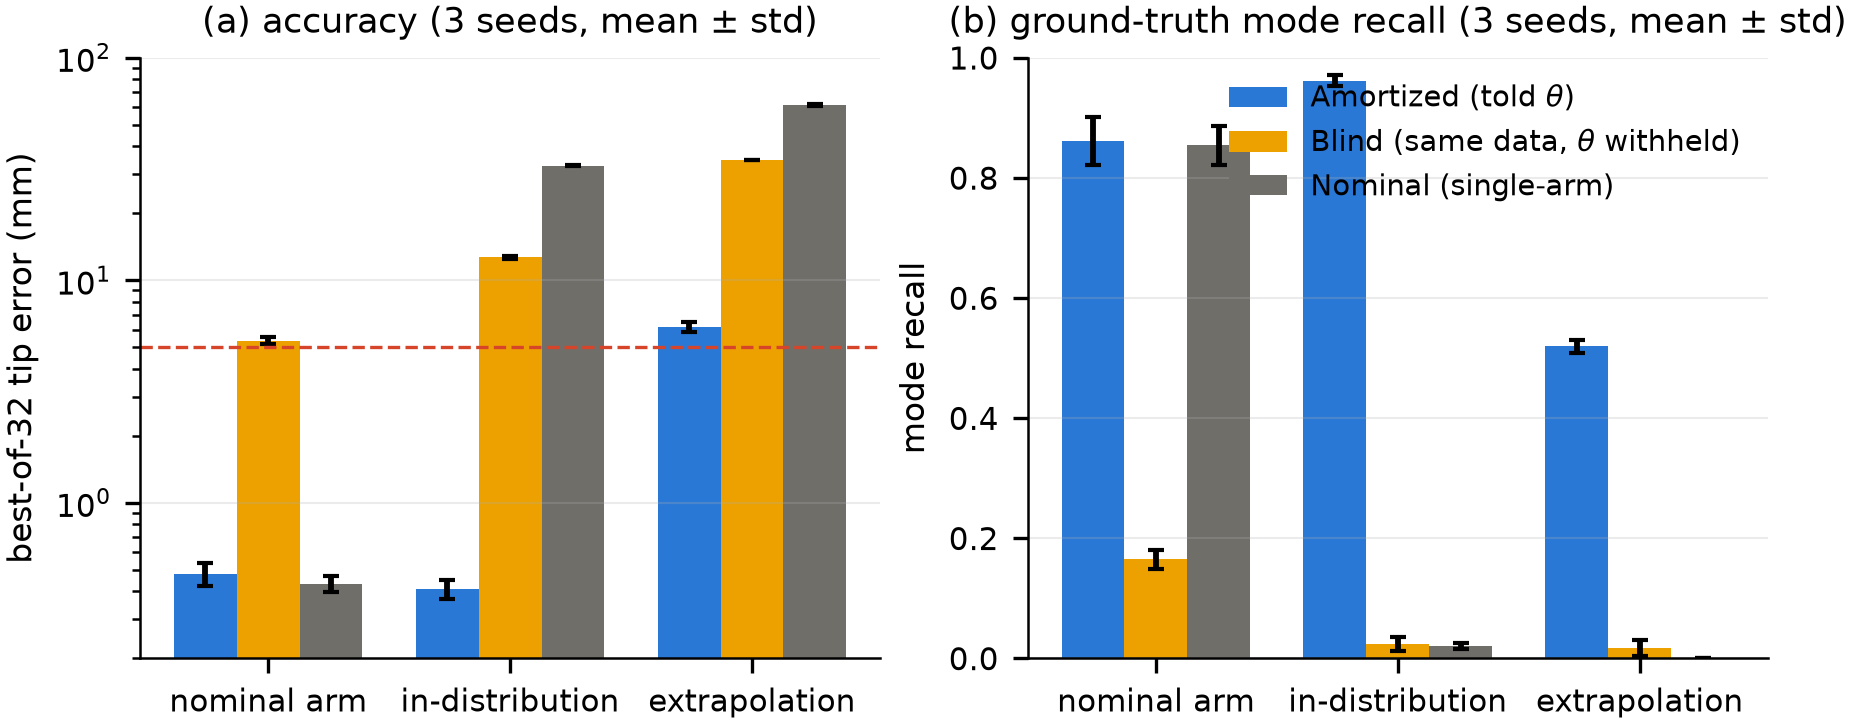
\includegraphics[width=\textwidth]{figures/fig_threeway.png}
\caption{The central comparison. (a) Best-of-32 tip error (log scale;
dashed line is the $5\,$mm success tolerance) and (b) ground-truth mode
recall, by test band, for the three models of Sec.~\ref{sec:design}.
Amortized and Blind share identical training data. Mean $\pm$ std over
three training seeds.}
\label{fig:threeway}
\end{figure}

\subsection{Amortization at the specialist's accuracy}

Table~\ref{tab:threeway} and Figure~\ref{fig:threeway} give the paper's
central result. On the five
held-out in-distribution morphologies, the amortized model reaches
$0.41\pm0.04\,$mm best-of-32 tip error with $100\%$ success on every arm
and every seed (per-seed means $0.40$, $0.46$, $0.37\,$mm; per-arm
three-seed means $0.31$--$0.56\,$mm). On the
nominal arm---which it never saw as an exact morphology---it reaches
$0.48\pm0.06\,$mm, against $0.43\pm0.04\,$mm for the specialist that
spent its entire $5\times10^5$-sample budget on that arm alone. The cost
of generalizing across the family, measured on the family's own nominal
member, is $0.05\,$mm---within one standard deviation, and $1\%$ of the
success tolerance.

A reviewer will ask whether that holds off the nominal arm, so we trained
a second specialist, on one of the held-out in-distribution morphologies
(single seed; $5\times10^5$ samples of that arm alone). It reaches
$0.33\,$mm; the amortized model on the same arm reaches $0.39\pm0.03\,$mm
(three seeds), with identical mode recall ($1.00$) and diversity ($21.1$
vs.\ $21.1$). The cost of amortization is $0.06\,$mm here and $0.05\,$mm
on the nominal arm: consistent, and a tenth of a percent of arm length.
Source: \texttt{results\_specialist\_indist0.json}.

The specialist, conversely, is useless off its arm: $32.8\pm0.2\,$mm and
$5\%$ success in-distribution, $61.1\pm0.7\,$mm and $0.4\%$
extrapolating. Its errors
on individual in-distribution arms range from $10$ to $65\,$mm; on the
long-segment arm, $115\,$mm. A model trained on one arm has learned a
lookup table for that arm, and the table is wrong everywhere else.

\subsection{The information, not the data}
\label{sec:blind}

The Blind model was trained on the identical samples as the Amortized
model. It reaches $12.68\pm0.21\,$mm and $12\%$ success
in-distribution---a $31\times$ gap in error, stable to $\pm0.2\,$mm across
seeds, attributable to nothing but the eight conditioning dimensions. On
the nominal arm it reaches $5.36\pm0.21\,$mm and $48\pm5\%$: training
on a randomized family \emph{without} the morphology lands worse than the
single-arm specialist on that very arm.

\begin{table}[H]
\caption{What the Blind model learned. For each sample $\mathbf{q}$ drawn
for target $\mathbf{t}$ on the queried arm: is it a valid solution
($<5\,$mm) on the queried arm, and is it valid on \emph{some} arm in the
training box (random search over $2\times10^4$ morphologies; a lower
bound, since the search rarely lands on any specific arm exactly)? 20
targets, 32 samples each; random actuations are the control. Seed 0.
Source: \texttt{results\_blind\_marginal.json}.}
\label{tab:marginal}
\begin{tabularx}{\textwidth}{llCC}
\toprule
\textbf{Queried arm} & \textbf{Samples from} & \textbf{valid on queried arm} & \textbf{valid on some arm} \\
\midrule
nominal      & Blind      & $2.2\%$  & $\mathbf{100.0\%}$ \\
             & Amortized  & $99.8\%$ & $100.0\%$ \\
             & random $\mathbf{q}$ & $0.0\%$ & $7.7\%$ \\
\midrule
in-dist      & Blind      & $0.0\%$  & $\mathbf{100.0\%}$ \\
             & Amortized  & $99.7\%$ & $96.1\%$ \\
             & random $\mathbf{q}$ & $0.0\%$ & $6.6\%$ \\
\midrule
extrap.\ stiff & Blind    & $0.0\%$  & $\mathbf{99.7\%}$ \\
             & Amortized  & $37.7\%$ & $40.0\%$ \\
             & random $\mathbf{q}$ & $0.0\%$ & $4.2\%$ \\
\bottomrule
\end{tabularx}
\end{table}

What did the Blind model learn instead? The hypothesis is that with the
morphology withheld, the model fits the marginal
$p(\mathbf{q}\,|\,\mathbf{t}) = \int p(\mathbf{q}\,|\,\mathbf{t},
\boldsymbol{\theta})\,p(\boldsymbol{\theta})\,d\boldsymbol{\theta}$:
every sample is a correct actuation for \emph{some} arm in the family,
and for the queried arm only by chance. This is testable, and
Table~\ref{tab:marginal} tests it. On every queried arm, essentially every
Blind sample ($99.7$--$100\%$) is a valid solution for some morphology in
the training box, while only $0$--$2\%$ are valid for the arm actually
queried. Random actuations pass the same search $4$--$8\%$ of the time,
so the test discriminates. The Blind model is not confused or
under-trained; it is a good sampler from the wrong distribution.

The prediction is quantitative. If each Blind sample is independently
valid on the nominal arm with probability $0.022$, best-of-32 success
should be $1-(1-0.022)^{32} = 51\%$; the measured rate is $48\pm5\%$
(Table~\ref{tab:threeway}). Blind's nonzero success is the chance that one
of 32 draws from the marginal happened to land on the queried arm.

This is the mechanism behind domain randomization's failure on this
problem. The finding that gain-DR degrades in-domain accuracy from $0.44$
to $2.18\,$mm and recovers nothing under model change
(Sec.~\ref{sec:transfer}) is the same effect, observed without the test
that explains it. DR does not fail because randomization is the wrong
idea; it fails because withholding the parameters turns a conditional
into a marginal, and a marginal over arms is not a solver for any of them.

The table's Amortized rows carry a second finding. In-distribution, an
amortized sample valid on the queried arm is also valid on some arm
($96\%$, the search's lower bound). On the extrapolated stiff arm, only
$40\%$ of amortized samples are valid \emph{anywhere} in the box: when
the model fails past its training family, its output is not a solution
for a neighbouring arm but a solution for none. Extrapolation failure is
breakdown, not confusion.

\subsection{The generalization envelope}
\label{sec:envelope}

\begin{figure}[H]
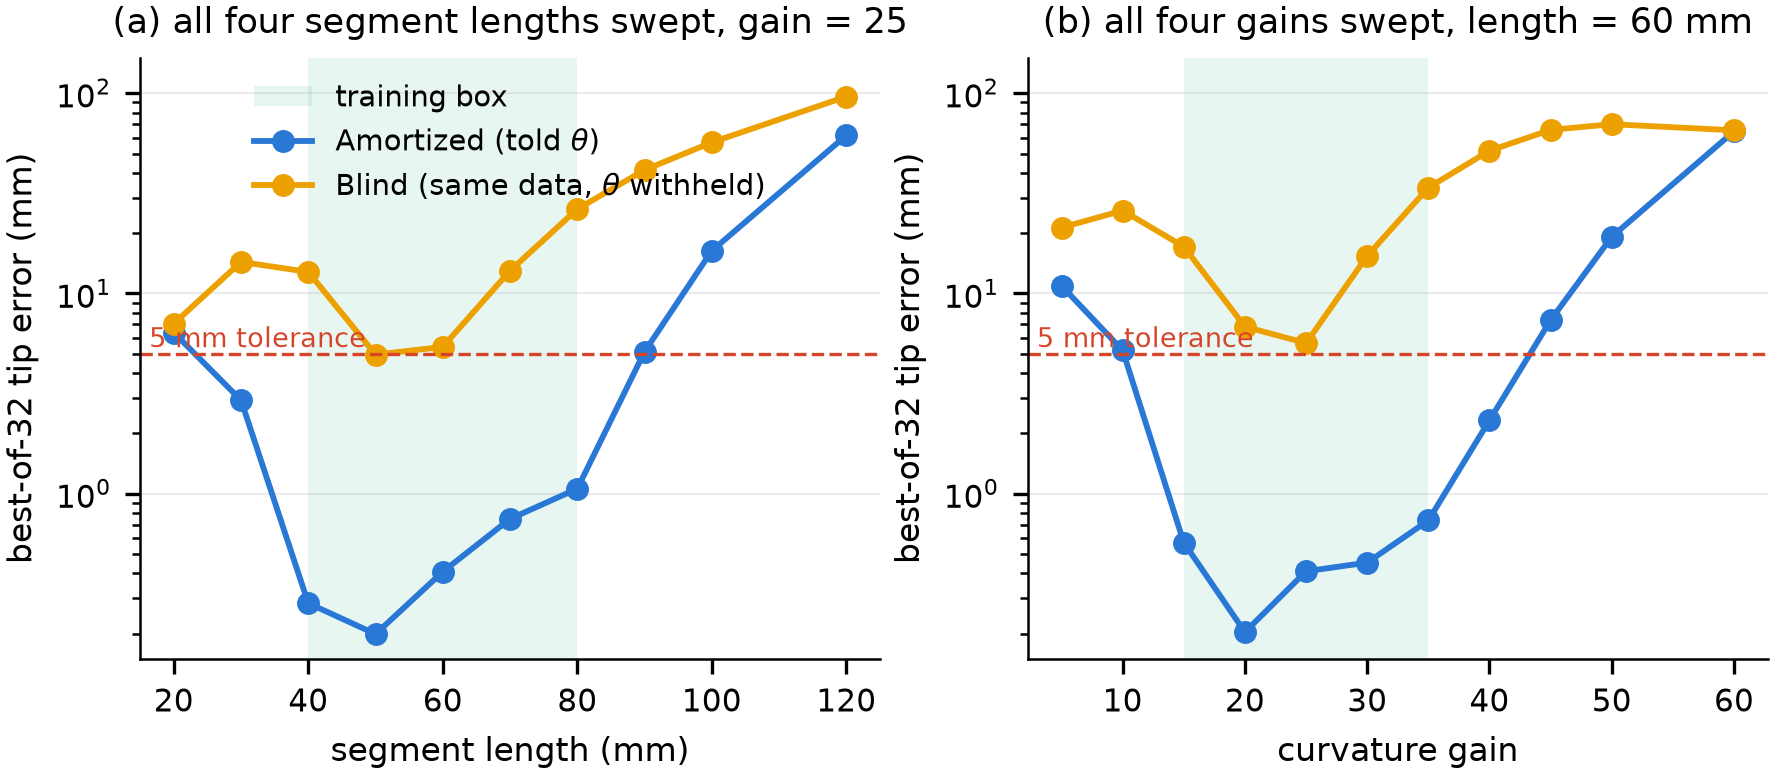
\includegraphics[width=\textwidth]{figures/fig_envelope.png}
\caption{Generalization envelope. One morphology axis is swept with the
other held at nominal, all four segments together; shaded region is the
training box. The amortized model is flat inside the box, degrades
gracefully just past its edge, then cliffs. The Blind model
is best at the box centre and worse toward every edge---the signature of a
model that learned the marginal over arms (Table~\ref{tab:marginal}).
Seed 0. Source:
\texttt{results\_envelope\_seed0.json}.}
\label{fig:envelope}
\end{figure}

\begin{table}[H]
\caption{Generalization envelope: one morphology axis swept with the other
at nominal, all four segments together. Best-of-32 error and success.
Shaded rows are inside the training box. Seed 0; source:
\texttt{results\_envelope\_seed0.json}.}
\label{tab:envelope}
\begin{tabularx}{\textwidth}{lCC|lCC}
\toprule
\multicolumn{3}{c|}{\textbf{Segment length (mm), $g{=}25$}} & \multicolumn{3}{c}{\textbf{Curvature gain, $L{=}60$}} \\
$L$ & Amortized & Blind & $g$ & Amortized & Blind \\
\midrule
20 & $6.4$ / $31\%$ & $7.1$ / $44\%$ & 5 & $10.9$ / $20\%$ & $21.3$ / $13\%$ \\
30 & $2.9$ / $94\%$ & $14.4$ / $1\%$ & 10 & $5.2$ / $56\%$ & $26.0$ / $12\%$ \\
\rowcolor{gray!12} 40 & $0.28$ / $100\%$ & $12.8$ / $7\%$ & \cellcolor{gray!12} 15 & \cellcolor{gray!12} $0.57$ / $100\%$ & \cellcolor{gray!12} $17.1$ / $14\%$ \\
\rowcolor{gray!12} 50 & $0.20$ / $100\%$ & $5.0$ / $57\%$ & \cellcolor{gray!12} 20 & \cellcolor{gray!12} $0.20$ / $100\%$ & \cellcolor{gray!12} $6.8$ / $36\%$ \\
\rowcolor{gray!12} 60 & $0.41$ / $100\%$ & $5.4$ / $50\%$ & \cellcolor{gray!12} 25 & \cellcolor{gray!12} $0.41$ / $100\%$ & \cellcolor{gray!12} $5.6$ / $41\%$ \\
\rowcolor{gray!12} 70 & $0.75$ / $100\%$ & $13.0$ / $12\%$ & \cellcolor{gray!12} 30 & \cellcolor{gray!12} $0.45$ / $100\%$ & \cellcolor{gray!12} $15.4$ / $6\%$ \\
\rowcolor{gray!12} 80 & $1.06$ / $99.6\%$ & $26.4$ / $1\%$ & \cellcolor{gray!12} 35 & \cellcolor{gray!12} $0.73$ / $99.6\%$ & \cellcolor{gray!12} $33.8$ / $1\%$ \\
90 & $5.1$ / $60\%$ & $41.4$ / $0.4\%$ & 40 & $2.3$ / $98\%$ & $51.7$ / $0\%$ \\
100 & $16.3$ / $3\%$ & $56.8$ / $0\%$ & 45 & $7.4$ / $30\%$ & $65.6$ / $0\%$ \\
120 & $61.6$ / $0\%$ & $96.2$ / $0\%$ & 50 & $19.2$ / $5\%$ & $70.1$ / $0\%$ \\
 & & & 60 & $64.5$ / $0\%$ & $65.3$ / $0\%$ \\
\bottomrule
\end{tabularx}
\end{table}

A single extrapolation number would mislead; what a reader needs is the
shape of the degradation. Figure~\ref{fig:envelope} and
Table~\ref{tab:envelope} sweep each axis from
well inside the box to well outside. Inside, the amortized model is flat:
$0.20$--$1.06\,$mm and $\geq 99.6\%$ success across the entire range of
both axes. Just past the edge it degrades gracefully---$L{=}90\,$mm
($12\%$ past) gives $5.1\,$mm at $60\%$; $g{=}40$ ($14\%$ past) gives
$2.3\,$mm at $98\%$---and then cliffs: $L{=}120\,$mm and $g{=}60$ are
$62$ and $65\,$mm at $0\%$.

The envelope is asymmetric. Shortening extrapolates further than
lengthening ($L{=}30\,$mm, $25\%$ below the box: $2.9\,$mm at $94\%$;
$L{=}90\,$mm, $12\%$ above: $5.1\,$mm at $60\%$), and stiffening further
than softening ($g{=}40$: $98\%$; $g{=}10$, $33\%$ below: $56\%$). Both
directions that extrapolate well shrink the workspace; both that
extrapolate poorly expand it into regions the training arms never reached.
The model generalizes over the morphology axis but not to tip positions
outside the union of training workspaces.

The Blind column is the marginal made visible: best at the box centre
($L{=}50$--$60\,$mm, $g{=}20$--$25$), where a draw from the marginal is
likeliest to be a draw for a nearby arm, worse toward every edge, and
never above $57\%$ success anywhere.

\subsection{Data efficiency}
\label{sec:data}

A single-arm specialist's accuracy as a function of its training-set size
is shown in Figure~\ref{fig:scaling}: $12.0\,$mm at $5\times10^3$
samples, $1.86$ at $2\times10^4$, $0.78$ at $5\times10^4$, $0.51$ at
$2\times10^5$, and $0.40\,$mm at $5\times10^5$. Reaching sub-millimetre
accuracy on one arm costs that arm $\sim$$5\times10^4$ samples; reaching
$0.4\,$mm costs it $5\times10^5$.

The amortized model spent $5\times10^5$ samples across a continuous 8-D
family---in expectation, zero samples at any specific morphology---and
reaches $0.41\pm0.04\,$mm on morphologies it never saw. Per arm served, its data
cost is not a number that can be written down: the family is a continuum.
What can be said is that one specialist's total budget buys specialist-level
accuracy on every arm in the box.

Amortization is not free at every budget. Trained on $10^5$ and
$2\times10^5$ total samples (single seed), the amortized model reaches
$1.36$ and $1.22\,$mm on held-out in-distribution arms, against $0.71$ and
$0.51\,$mm for a specialist given the same total on its own arm---roughly
$2\times$ worse, while still at $\geq 99\%$ success. At $5\times10^5$ the
two converge ($0.39$ vs.\ $0.40\,$mm). Spreading a small budget over a
family costs accuracy; spreading a large one does not. The crossover lies
between $2\times10^5$ and $5\times10^5$ total samples for this family.

\begin{figure}[H]
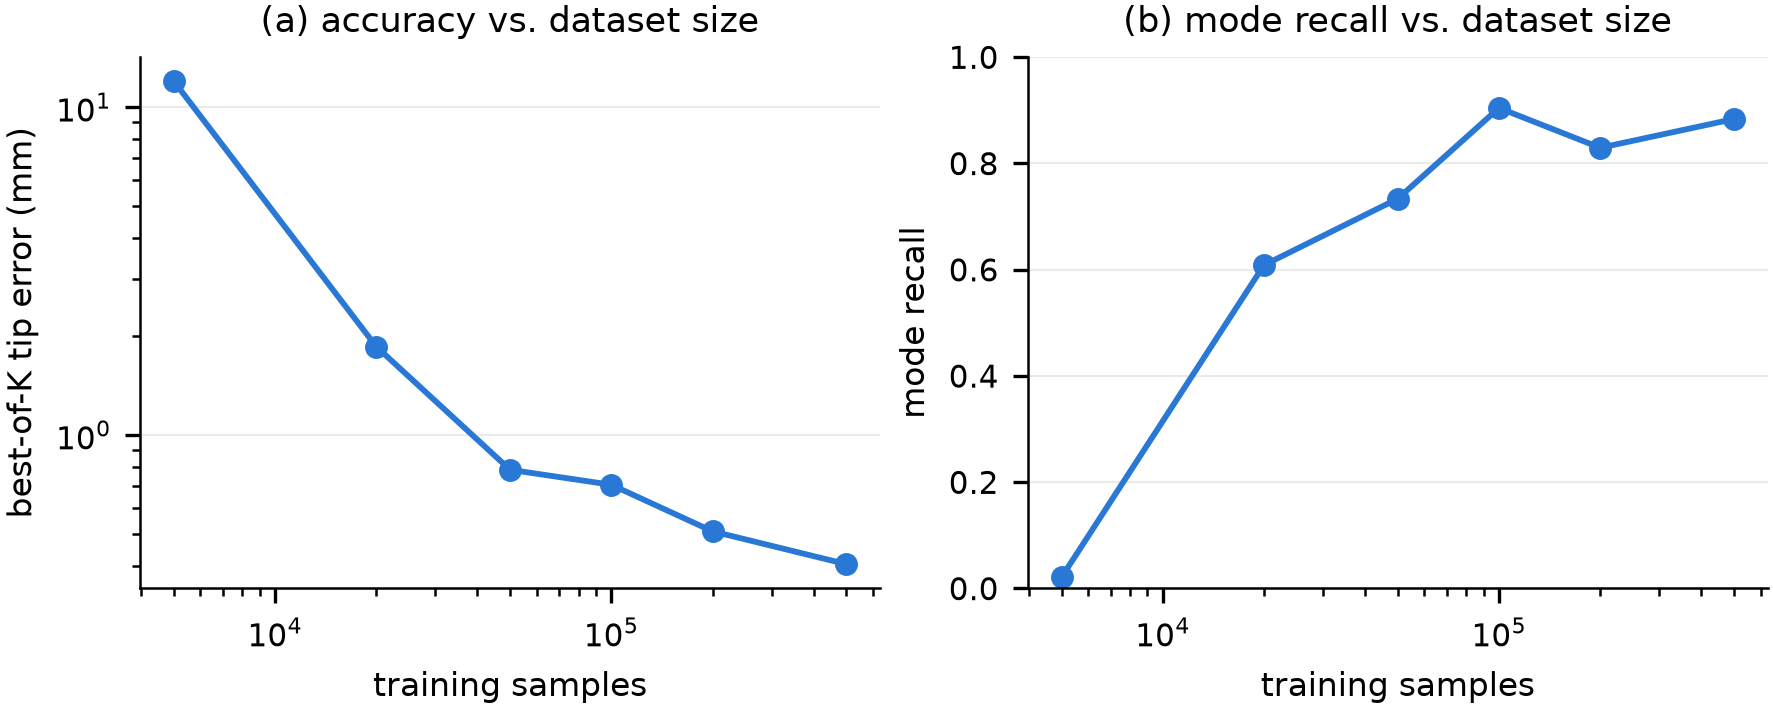
\includegraphics[width=0.8\textwidth]{figures/fig_scaling.png}
\caption{Single-arm dataset-size ablation on the nominal arm (single seed).
(a) Best-of-$K$ tip error and (b) mode recall vs.\ training-set size;
both saturate by ${\sim}0.5$--$1\times10^5$ samples. The amortized model
reaches the $5\times10^5$-sample specialist's accuracy on every
in-distribution arm with the same total budget spread across the family.}
\label{fig:scaling}
\end{figure}

\subsection{Multimodality under amortization}
\label{sec:modes}

\begin{table}[H]
\caption{Mode recall and solution diversity on held-out morphologies,
against ground-truth solution sets enumerated on each test arm ($2\times10^6$
sweep, DBSCAN in curvature space; 20 targets per arm, successful samples
only). Nominal band is one arm; in-distribution is five held-out arms;
extrapolation is the three of five arms on which enumeration found modes
(see text). Enumerated modes per target: nominal $2.05$; in-distribution
$1.00$--$1.90$. Mean $\pm$ std over three training seeds. Source:
\texttt{results\_morph\_3seed.json}.}
\label{tab:modes}
\begin{tabularx}{\textwidth}{lCCCCCC}
\toprule
 & \multicolumn{2}{c}{\textbf{Amortized}} & \multicolumn{2}{c}{\textbf{Blind}} & \multicolumn{2}{c}{\textbf{Nominal}} \\
\textbf{Band} & recall & div. & recall & div. & recall & div. \\
\midrule
Nominal arm     & $\mathbf{0.86\pm0.04}$ & $27.4\pm0.5$ & $0.17\pm0.02$ & $5.0\pm1.6$ & $0.85\pm0.03$ & $\mathbf{28.1\pm0.2}$ \\
In-distribution & $\mathbf{0.96\pm0.01}$ & $\mathbf{25.0\pm0.2}$ & $0.02\pm0.01$ & $0.2\pm0.3$ & $0.02\pm0.01$ & $0.2\pm0.2$ \\
Extrapolation   & $\mathbf{0.52\pm0.01}$ & $\mathbf{6.4\pm0.6}$ & $0.02\pm0.01$ & $0.0$ & $0.00$ & $0.0$ \\
\bottomrule
\end{tabularx}
\end{table}

The single-arm advantage was a multimodality advantage
(Table~\ref{tab:single}). Whether amortization preserves it---whether the
model still recovers the distinct solution modes of an arm it never
saw---decides whether the amortized model is an IK \emph{solver} or merely
an IK \emph{regressor} that happens to be conditioned well.
Table~\ref{tab:modes} answers: it is a solver. On held-out in-distribution
arms the amortized model recovers $0.96\pm0.01$ of enumerated modes with
sampled diversity $25.0\pm0.2$ in curvature space. The Blind model
recovers essentially none ($0.02\pm0.01$): a sampler from the marginal
does not merely miss the target, it misses every mode of every arm.

The in-distribution recall should not be read as exceeding the
specialist's on its own arm ($0.85\pm0.03$). The five in-distribution
arms average fewer enumerated modes per target ($1.00$--$1.90$; mean
$1.35$) than the nominal arm ($2.05$), and recall falls with mode count
across them (from $1.00$ on the one-mode arm to $0.88$ on the $1.9$-mode
arm). On the nominal arm itself, where the mode count is matched, the
amortized and specialist models are indistinguishable ($0.86\pm0.04$ vs.\
$0.85\pm0.03$). The fair statement is that amortization preserves mode
recall at the specialist's level; it does not raise it.

In extrapolation, recall tracks success arm by arm: $0.88$ recall at
$92\%$ success on the short arm, $0.58$ at $55\%$ on the compliant arm,
$0.09$ at $8\%$ on the mixed arm. Past the training box the model does not
find one solution while missing the others; when it reaches a target it
recovers that target's modes, and when it fails it fails entirely---the
breakdown of Table~\ref{tab:marginal}, seen from the mode side. The
diversity figure for this band ($6.4\pm0.6$) is low chiefly because
diversity is computed over successful samples and the mixed arm
contributes almost none. (Two of the five extrapolation arms---all-long
and all-stiff---are excluded from the recall average because the
enumeration itself found no modes on them: the DBSCAN scale was calibrated
to the nominal arm's curvature range, and those two arms move furthest
from it. The model reaches $97\%$ success on the stiff arm, so this is an
enumeration limit, not a model failure; see Sec.~\ref{sec:limitations}.)

\subsection{Only a multimodal model amortizes}
\label{sec:arch}

\begin{table}[H]
\caption{Architecture comparison under amortization: all three models
conditioned on $[\text{tip},\boldsymbol{\theta}]$ and trained on the same
data. Best-of-32 error and success, seed 0. Source:
\texttt{results\_morph\_seed0.json}.}
\label{tab:arch}
\begin{tabularx}{\textwidth}{lCCC}
\toprule
\textbf{Band} & \textbf{Diffusion} & \textbf{MLP} & \textbf{MDN} \\
\midrule
Nominal arm     & $\mathbf{0.42}$ / $100\%$ & $13.8$ / $1\%$ & $18.1$ / $2\%$ \\
In-distribution & $\mathbf{0.39}$ / $100\%$ & $14.1$ / $3\%$ & $16.3$ / $5\%$ \\
Extrapolation   & $\mathbf{6.2}$ / $61\%$ & $31.8$ / $15\%$ & $20.8$ / $18\%$ \\
\bottomrule
\end{tabularx}
\end{table}

Given the morphology, does any architecture amortize? Table~\ref{tab:arch}
says no. The MLP and MDN, trained on the identical morphology-conditioned
data, reach $14.1$ and $16.3\,$mm in-distribution---no better than their
single-arm performance in Table~\ref{tab:single}, and no better than they
manage without the morphology at all. The conditioning is not the
bottleneck for them; their inability to represent a multimodal conditional
is. Amortizing over morphology does not reduce the multimodality of the
inverse map---it adds a dimension along which the solution set varies---so
the models that could not represent it on one arm cannot represent it on a
family. Diffusion's advantage under amortization is not a capacity
advantage: the MLP and MDN are matched in width, and the MLP's validation
loss on its own objective decreases monotonically to convergence. It fits
the conditional mean as well as it can; the mean is not a solution.

% =========================================================================
\section{The Advantage Is Redundancy, Specifically}
\label{sec:mechanism}
% =========================================================================

If diffusion's advantage---on one arm or on a family---is redundancy
resolution, it should shrink when redundancy is removed and grow when it is
added. Both predictions hold on one arm (Figure~\ref{fig:redundancy}), and
the amortization results extend the second.

\begin{figure}[H]

\includegraphics[width=\textwidth]{figures/fig_redundancy.png}
\caption{The diffusion advantage tracks actuation redundancy. (a) Replacing
the 3-D tip target with a 24-D whole-shape target removes most of the
redundancy: sampled diversity collapses ${\sim}80\times$ ($28.16\pm0.22$ to
$0.346\pm0.022$; 3 seeds). (b) Increasing the number of segments (single
seed per morphology) widens the diffusion--MLP accuracy gap monotonically
from two to ten segments; from eight segments on, the MLP's obstacle-task
success is $0\%$ while diffusion's stays ${\geq}99.5\%$.}
\label{fig:redundancy}
\end{figure}

\textbf{Removing redundancy.} Conditioning on the full 24-D body shape
instead of the 3-D tip pins down almost the whole configuration. Diffusion's
sampled diversity collapses from $28.16\pm0.22$ to $0.346\pm0.022$
(${\sim}80\times$), and the MLP's accuracy disadvantage shrinks from
${\sim}30\times$ to ${\sim}3\times$ ($0.49$ vs.\ $0.16\,$mm per-point
error, both at $100\%$ success, 3 seeds). When there is one answer, a
deterministic regressor is nearly as good.

\textbf{Adding redundancy.} Across two-, six-, eight-, and ten-segment
arms (single seed each), the MLP's error grows monotonically from $1.7$ to
$103.2\,$mm with $0\%$ success from eight segments on, while diffusion
degrades gracefully ($0.11$ to $3.2\,$mm, $\geq 99.8\%$ success). Amortizing
over morphology is a third way of adding redundancy---the same tip is now
reachable by different shapes on different arms---and Sec.~\ref{sec:arch}
shows the same ordering: the deterministic models fail, the multimodal one
does not.

% =========================================================================
\section{Under Dynamics-Model Change}
\label{sec:transfer}
% =========================================================================

Amortization across morphology is generalization across \emph{parameters
of the same model}. It is a different question whether a learned inverse
map survives a change of \emph{dynamics model}---executing PCC-trained
actuations on a Cosserat-rod simulation of the same arm (PyElastica,
48 elements, $1.5\,$s damped horizon;~\cite{gazzola2018forward,zhang2019modeling}).
It does not: accuracy collapses from $0.67\pm0.03$ to $139.9\pm1.8\,$mm
with $0\%$ success on every seed ($n{=}20$ held-out targets, $K{=}8$; the
PCC-domain figure differs from Table~\ref{tab:single}'s $0.44\,$mm only
by this smaller $K$), and the discrepancy is
directional---no couple gain or damping constant aligns the two workspaces.

We characterized what recovers this loss and what does not;
Table~\ref{tab:synthesis} summarizes and Figures~\ref{fig:budget}
and~\ref{fig:cliff} give the two central curves.
Selection under an Elastica query budget improves every target but never
solves one; a diversity-aware query ordering significantly beats a
confidence ordering (paired $t{=}3.34$, $p{\approx}0.002$); guided
sampling is suggestive at best; fine-tuning on $10^4$ target-domain samples
yields the only nonzero success ($67.1\pm0.9\,$mm, $10\%$) at the price of
catastrophic forgetting, and mixing source data back in collapses the gain
below the first grid point---a retention--transfer cliff with no sweet spot.

\begin{figure}[H]
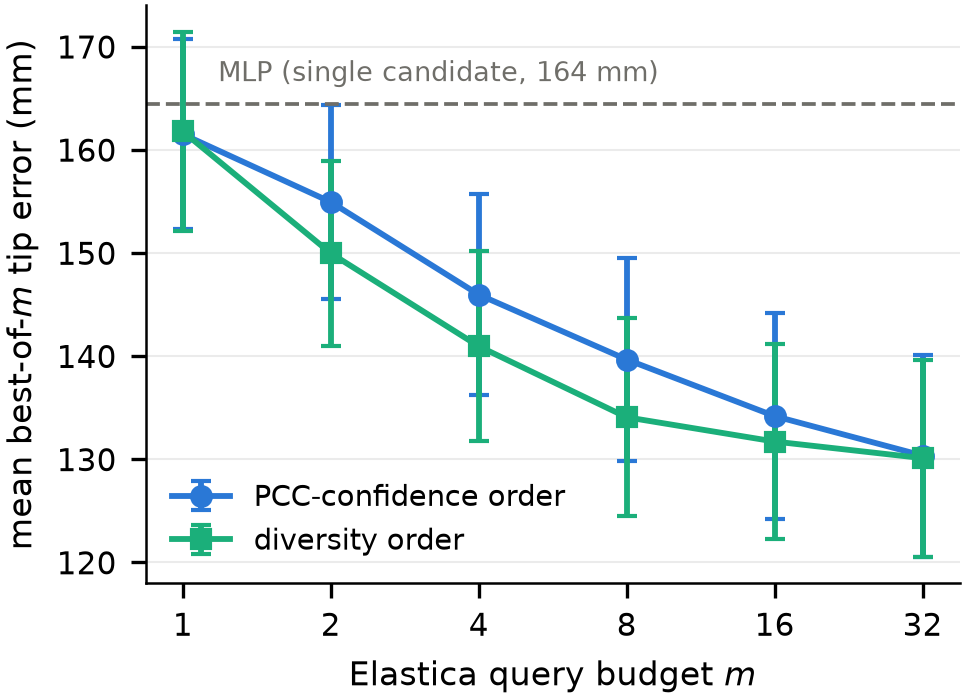
\includegraphics[width=0.8\textwidth]{figures/fig_query_budget.png}
\caption{Candidate selection under an Elastica query budget ($n{=}45$
targets, $K{=}32$ candidates, mean $\pm$ SEM). A diversity-aware
(farthest-point) ordering of which candidates to evaluate beats a
confidence ordering; in the paired design the difference is significant at
$m{=}8$ and $m{=}16$ ($t{=}3.34$ and $3.21$, $p{\approx}0.002$).}
\label{fig:budget}
\end{figure}

\begin{figure}[H]
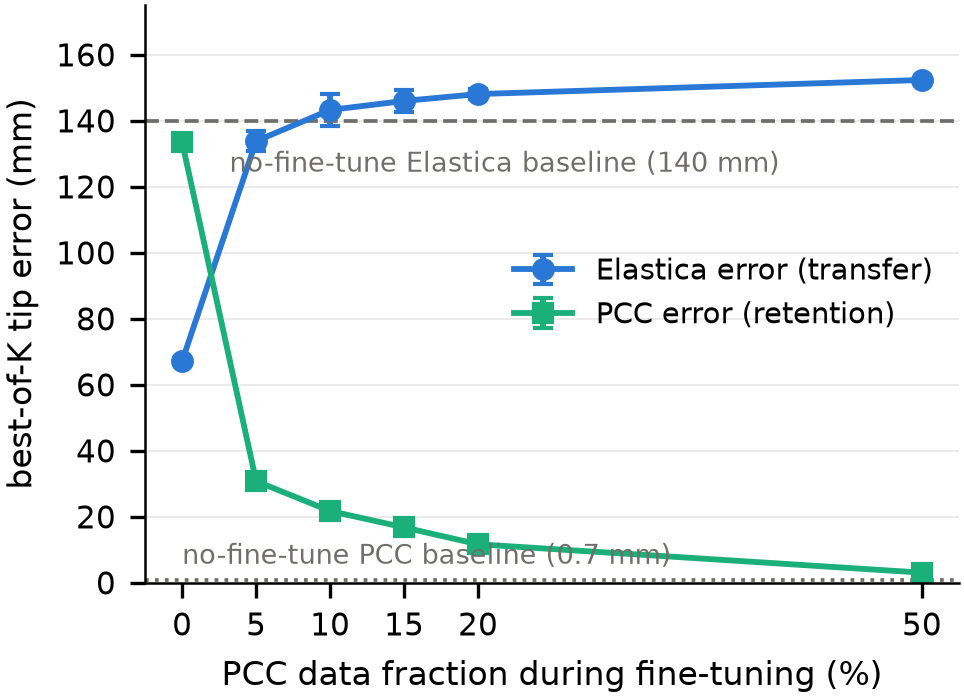
\includegraphics[width=0.8\textwidth]{figures/fig_finetune_cliff.png}
\caption{The retention--transfer cliff (mean $\pm$ std, 3 seeds; six
mixing ratios). Fine-tuning on $10^4$ Elastica samples: retention improves
smoothly as source data is mixed back in, but the transfer gain collapses
almost entirely by the first grid point ($5\%$). There is no sweet spot.}
\label{fig:cliff}
\end{figure}

\begin{table}[H]
\caption{Recovery mechanisms under dynamics-model change (Elastica-domain
performance; best configuration of each; each row on its own held-out
target set, 15--45 targets).}
\label{tab:synthesis}
\begin{tabularx}{\textwidth}{lCCl}
\toprule
\textbf{Mechanism} & \textbf{err (mm)} & \textbf{succ.} & \textbf{Cost / caveat} \\
\midrule
none (top-1 candidate) & $161.5$ & $0\%$ & no target queries \\
best-of-32 selection & $130.4$ & $0\%$ & 32 queries/target \\
\; + diversity order & $-6.7$ at $m{=}8$ & $0\%$ & same queries; $p{\approx}0.002$ \\
guided sampling & $129.0$ & $0\%$ & 400 labels; suggestive \\
gain randomization (blind) & $140.6$ & $0\%$ & degrades source; no gain \\
fine-tune, $0\%$ mix & $\mathbf{67.1\pm0.9}$ & $\mathbf{10\%}$ & forgets source ($133\,$mm) \\
fine-tune, $\geq 5\%$ mix & $\geq 133.8$ & $\leq 10\%$ & retains source, forfeits gain \\
\bottomrule
\end{tabularx}
\end{table}

The row labelled \emph{gain randomization} is the one this paper
reinterprets. It was reported as a null result: randomizing the gain buys
nothing. Sec.~\ref{sec:blind} shows why. That model was Blind; it had
learned the marginal over gains, and a sample from that marginal is no
likelier to suit the Cosserat arm than one from the nominal model. Whether an \emph{Amortized} model---one that has
learned the inverse map as a function of morphology---can be steered
toward the Cosserat arm by inferring an effective morphology for it is the
natural next question, and one this paper's machinery makes askable. It
is not answered here.

% =========================================================================
\section{Discussion}
% =========================================================================

\textbf{What amortization buys.} A practitioner with a fabricated soft arm
whose segment lengths and gains can be measured---or estimated from a
handful of calibration poses---can use one pretrained model rather than
train one. The accuracy cost is under a tenth of a millimetre inside the
training family and modest for the first $10$--$15\%$ beyond it. Because the conditioning is a continuous
vector, the model would also support a mode of use no per-arm model can:
sweeping $\boldsymbol{\theta}$ at a fixed target to ask which morphology
in the family reaches it most easily. We note the possibility; this paper
does not evaluate it.

\textbf{Why the ablation matters.} That conditioning on identified
parameters beats marginalizing over them is the premise of universal
policies~\cite{yu2017preparing}. What the Blind result adds is a
controlled measurement of the cost of marginalizing, on a problem where
the conditional is multimodal: identical data, one conditioning vector
removed, a $31\times$ accuracy gap, and a direct test
(Table~\ref{tab:marginal}) showing the marginal was learned faithfully.
The practical consequence is direct: when the randomized parameters can be
observed at deployment, they should be conditioned on, not marginalized
over. DR is the right tool only when the parameters are genuinely
unobservable, and its cost in that case---a sampler whose every draw is
right for some arm and wrong for yours---should be budgeted for.

\textbf{Why only diffusion.} The MLP's converged fit alongside its
$14\,$mm error is the cleanest statement of the paper's mechanism. A model
that fits the conditional mean can fit it arbitrarily well and still return
an actuation that is not a solution, because the solutions are a set and
the mean of a set is not in it. Amortization makes the set larger.

\textbf{Relation to rigid-robot amortization.} IKDiffuser~\cite{zhang2025ikdiffuser}
amortizes over discrete kinematic-tree topologies by tokenization. The soft
case differs in that the morphology is a continuous parameter of a single
topology, which makes interpolation and extrapolation meaningful
notions---and we are not aware of a comparable envelope measurement for
a generative IK model on any robot.

% =========================================================================
\section{Limitations}
\label{sec:limitations}
% =========================================================================

(1) \textbf{Simulation only.} Every result is on a simulated arm; no claim
is made about hardware. The motivating fabrication-variability argument is
a reason to want amortization, not evidence that this model delivers it on
a physical arm. (2) \textbf{The morphology must be known.} The amortized
model is conditioned on $\boldsymbol{\theta}$; it does not infer it. On a
physical arm the eight parameters would have to be measured or calibrated,
and the model's sensitivity to error in them is not characterized here.
(3) \textbf{One segment count.} The family varies lengths and gains at
fixed $N{=}4$; segment count changes the actuation dimension and is
outside this study's conditioning scheme. (4) \textbf{Statistical
coverage.} The single-arm comparison, shape-conditioning, transfer
collapse, fine-tuning grid, the central amortization comparison
(Table~\ref{tab:threeway}), and held-out mode recall (Table~\ref{tab:modes})
carry three-seed statistics. The query-budget, ordering, guidance,
hyperparameter, segment-count, envelope-sweep, architecture-comparison,
amortized-scale, marginal-test, and second-specialist results are
single-seed. (5) \textbf{Extrapolation is bounded.} The model
does not generalize to tip positions outside the union of training
workspaces; the cliff in Table~\ref{tab:envelope} is a real boundary, not
a tail. (6) \textbf{Dynamics-model change is not solved.} Sec.~\ref{sec:transfer}
is an honest boundary on what any learned inverse map in this family can
currently do. (7) \textbf{Mode enumeration does not reach every arm.} The
DBSCAN parameters were calibrated on the nominal arm; on the two
extrapolation arms whose curvature-space scale is furthest from it,
enumeration found no ground-truth modes and recall is undefined there.
(8) \textbf{The test suite is eleven arms.} Five in-distribution draws and
five extrapolation cases along chosen axes; the envelope sweeps one axis at
a time with the other at nominal. Joint extrapolation on both axes is
represented by a single mixed case. (9) \textbf{The marginal test is a
lower bound.} Random search over $2\times10^4$ morphologies rarely lands on
any specific arm, so ``valid on some arm'' understates; the Blind rows are
at $100\%$ regardless.

% =========================================================================
\section{Conclusions}
% =========================================================================

One conditional diffusion model, told which arm it is solving for,
solves inverse kinematics for an entire continuous family of soft
continuum arms---within a tenth of a millimetre of a per-arm specialist,
with no data from any specific arm, and with graceful degradation for a
measured distance beyond the family it was trained on. The same data with the morphology
withheld does not: it learns the marginal over the family, every sample
a solution for some arm and almost none for the one queried---measured
directly, and predicting the observed success rate. Domain randomization's
failure on this problem is an information failure, and the ablation that
shows it changes nothing but eight conditioning dimensions. Only a
model that represents the multimodal solution set can exploit that
information, because under amortization the solution set varies with
morphology as well as with target. For
learned soft-arm IK, the path past the single-arm model is not more data
from that arm but a model conditioned on which arm it is.

\vspace{6pt}

\funding{This research received no external funding.}

\dataavailability{All code, configuration, per-experiment result files, and
training-data generators are publicly available at
\url{https://github.com/adhvayjagadeesh/soft-arm-diffusion-ik}. Every
number in this paper traces to a committed result file named in its table
caption, and \texttt{scripts/print\_paper\_tables.py} regenerates the
amortization tables from them.}

\acknowledgments{During the preparation of this study and manuscript, the
author used Claude (Anthropic; Claude Opus 5, via Claude Code) for the
purposes of drafting and editing text, writing and running experiment and
analysis code, generating figures, and checking reported numbers against
result files. The author has reviewed and edited the output and takes full
responsibility for the content of this publication.}

\conflictsofinterest{The author declares no conflicts of interest.}

\begin{adjustwidth}{-\extralength}{0cm}
\reftitle{References}
\externalbibliography{yes}
\bibliography{references}
\PublishersNote{}
\end{adjustwidth}

\end{document}
